\input{header}
\physics
\begin{document}
\papertitle{Determination of \textit{g} through precession of an air gyroscope}
\paperauth{A}{Khesin}{1002442029}
\paperauth{P}{Zavyalova}{1002345036}
\paperdate{March 28, 2018, Completed March 22, 2018}
\begin{paperabs}

	Abstract goes here
	
\end{paperabs}

\begin{paper}
	
\papersec{Introduction}
	
	The value of \textit{g} may be accurately determined by examining the precession of a gyroscopic rotator, an accurately machined sphere with a flat region. The sphere is driven by a coil to rotate with the axis of rotational symmetry horizontal. The rotator ends up being magnetized along an equatorial diameter and therefore together with the coil constitutes a synchronous motor. Since the rotor is free, the angular momentum vector may freely change its direction. 
	
	The change in the angular momentum vector of the rotor arises from a torque acting in the horizontal plane resulting from the imbalance from the truncated section of the sphere. A pure precession about a vertical axis arises due to the fact that the torque is at all times perpendicular to the angular momentum. 
	
	In this experiment, the above setup was implemented with the goal of approximating \textit{g}. Constant torsion-free air suspension supported the sphere. The rotor was accelerated using a controllable air flow until a frequency of \( 3600 \) rpm was attained. The frequency of rotation was measured using a strobe light; as soon as the desired value was obtained, the accelerating air flow was shut off and the driving coil was switched on. The rotator was driven at \( \pars{60 \pm .1} \si{\hertz} \) by a coil connected to the A.C. mains. To determine the period of rotation of the sphere, a laser light was reflected from the surface of the sphere. By marking the position of a well-defined spot resulting from specular reflection from the flat section and measuring the time of a full revolution, the period was obtained. The complete experimental setup is shown below.
	
	\paperfig{Setup}{\pdf{setup} \vspace{-2.5em}}{Experimental setup used for determining the value of \textit{g} through precession of an air gyroscope. The driving coil was mounted in the platform supporting the truncated sphere, a laser was aligned with the flat surface, and a strobe light was used to ensure that the desired frequency is maintained.}
	
	Expressions for torque \( L \) and moment of inertia of the rotator may be calculated by assuming a uniform density of the sphere. The dimensions of the gyroscopic rotator were denoted as follows. 
	
	\paperfig{Sphere}{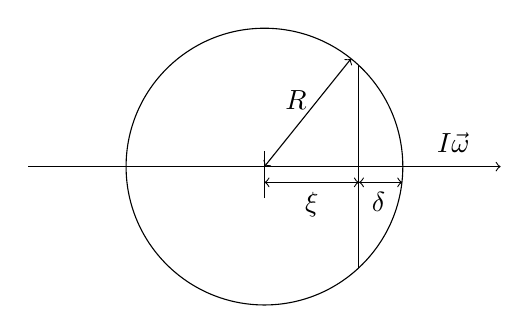
\begin{tikzpicture}
		\draw (0, 0) circle (50pt);
		\draw[->] (-3, 0)--(3, 0);
		\draw[-] (1.2, -1.29)--(1.2, 1.29);
		\draw[<->] (0, 0)--(1.1, 1.37);
		\draw[-] (0, -0.4)--(0, 0.2);
		\draw[<->] (0, -0.2)--(1.2, -0.2);
		\draw[<->] (1.2, -0.2)--(1.75, -0.2);
		\draw (0.6, -0.2) node[below] {\( \xi \)};
		\draw (1.45, -0.2) node[below] {\( \delta \)};
		\draw (0.4, 0.6) node[above] {\( R \)};
		\draw (2.4, 0.3) node {\( I\vec{\omega} \)};
	\end{tikzpicture}}{A sphere of radius \( R \) truncated to obtain a minimum distance from the center of \( R - \delta = \xi \), constituting a gyroscopic rotator. The angular momentum vector lies in the horizontal plane at all times and has a magnitude of \( I\omega \)}.

\papersec{Observations}
	
	Observations go here
	
\papersec{Analysis} 
	
	Analysis goes here

\papersec{Conclusion}

	Conclusion goes here
	
\papersec{Sources}

	\papersource{}

\end{paper}
\end{document}